% ----------------------------------------

\subsection{Contextual hypotesis}

% ----------------------------------------

\begin{frame}

\frametitle{Scenario}

In this case the e-commerce website doesn't register neither the \textbf{units sold} for each product nor the \textbf{class parameters}.

\todo{expand}

\end{frame}

% ----------------------------------------

\subsection{Algorithm}

% ----------------------------------------

\begin{frame}

\frametitle{Algorithm}
\framesubtitle{Algorithm outline}

so in order to work it estimate the list of values, corresponding to the earnings for each product given the knowledge obtained by the learner until now
We separately consider all the aggregated interactions where users landed on a certain product, then compute the reward they generated.
This way we obtain reward associated to a single campaign.

\todo{expand and correct}

\end{frame}

% ----------------------------------------

\subsection{Results}

% ----------------------------------------

\begin{frame}[plain]

\frametitle{Single run reward and regret}
\framesubtitle{Thompson Sampling and UCB}

\begin{center}
	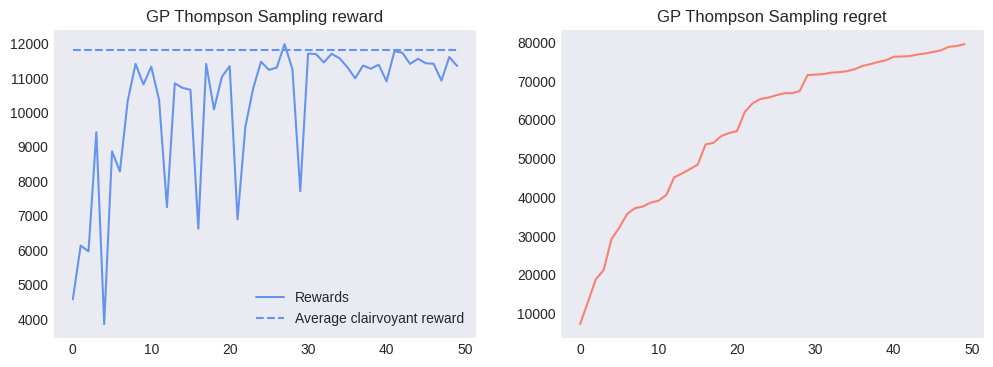
\includegraphics[scale=0.4]{img/Graphs/uncertain_alpha_unit/image1.png}
	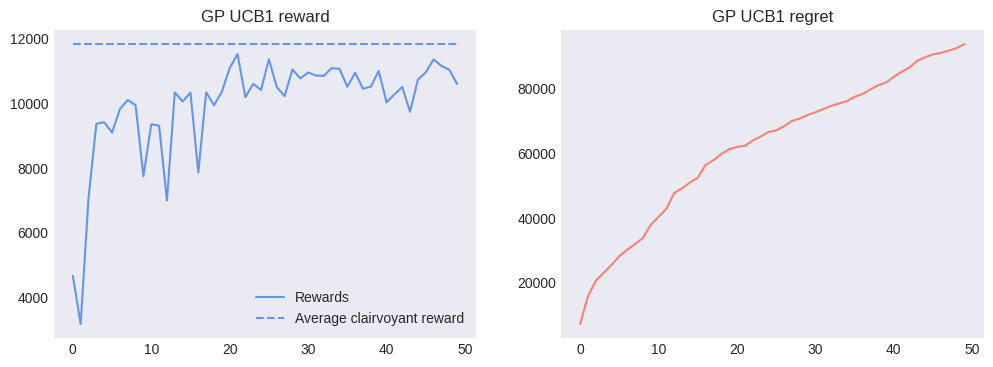
\includegraphics[scale=0.4]{img/Graphs/uncertain_alpha_unit/image2.png}
\end{center}

\end{frame}

% ----------------------------------------

\begin{frame}[plain]

\frametitle{Regret comparison}
\framesubtitle{Thompson Sampling and UCB}

\begin{center}
	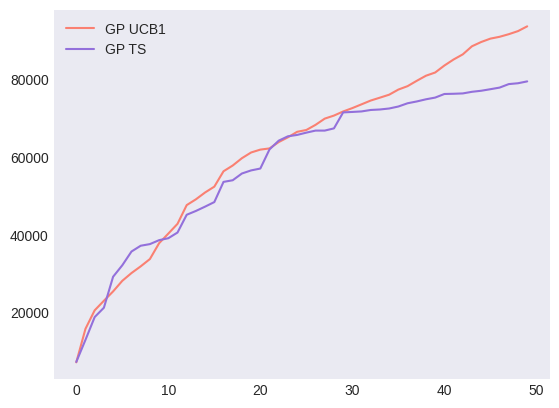
\includegraphics[scale=0.5]{img/Graphs/uncertain_alpha_unit/image3.png}
\end{center}

\scriptsize All tests are done using the \texttt{example\_environment} default values, \textit{population mean} of 1000, \textit{variance} of 10 and 20 \textit{budget steps}.

\end{frame}

% ----------------------------------------

\begin{frame}[plain]

\frametitle{Average regret and reward}
\framesubtitle{Thompson Sampling and UCB}

\begin{center}
	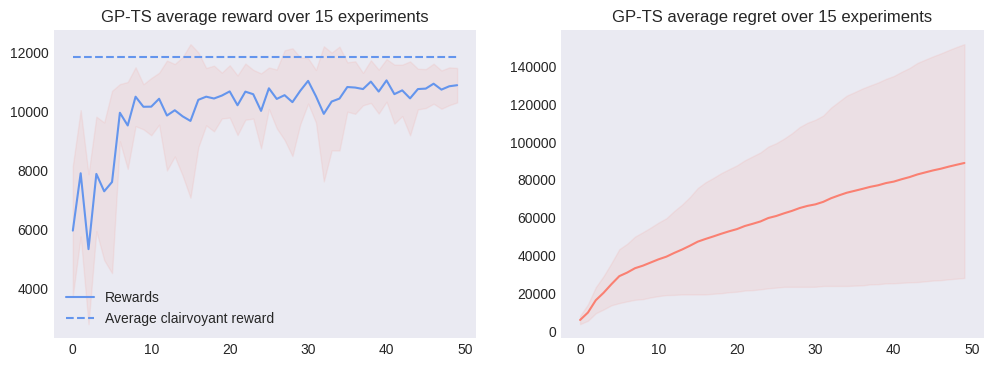
\includegraphics[scale=0.4]{img/Graphs/uncertain_alpha_unit/image4.png}
	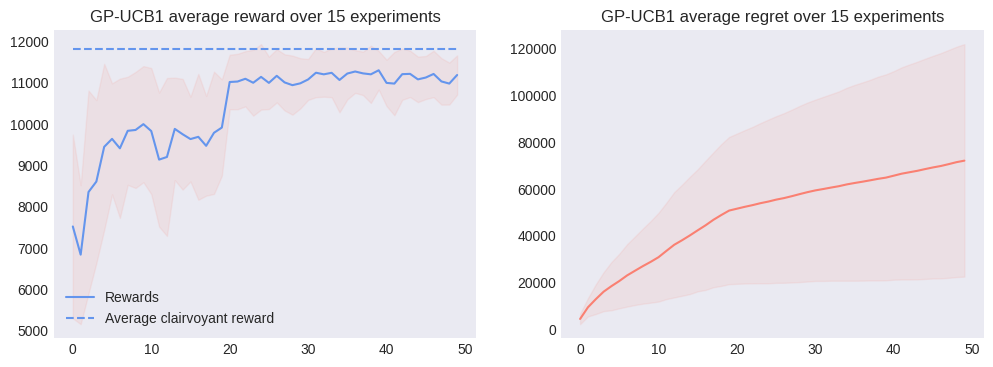
\includegraphics[scale=0.4]{img/Graphs/uncertain_alpha_unit/image5.png}
\end{center}

\end{frame}

% ----------------------------------------

\begin{frame}[plain]

\frametitle{Average regret comparison}
\framesubtitle{Thompson Sampling and UCB}

\begin{center}
	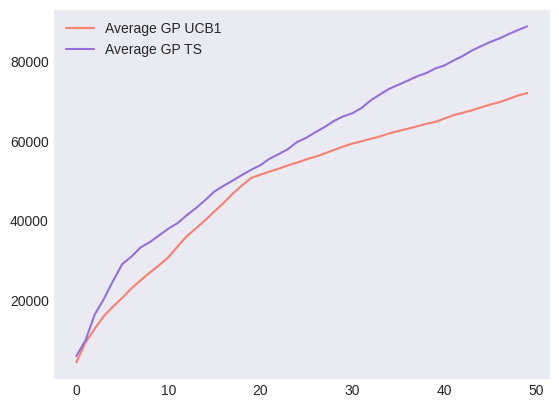
\includegraphics[scale=0.45]{img/Graphs/uncertain_alpha_unit/image6.png}
\end{center}

\begin{displaymath}
	\text{Regret ratio } = \frac{\text{Avg regret}}{\text{Upper bound}} = \frac{31019.4}{?} = ?
\end{displaymath}

\scriptsize Values reference GPTS regret compared to advertising GP regret found at [SLIDE REFERENCE]

\todo{complete}

\end{frame}

% ----------------------------------------

\begin{frame}

\frametitle{Results}

In this scenario, results are worse w.r.t. the previous step since the learners work with less information.

\textbf{TS} seems to reach the optimal solution but is much more unstable than the previous case, however, if we use the \textbf{UCB} approach we are not guaranteed to find the optimal arm as sometimes it settles on a suboptimal solution.

On average we can observe that \textbf{UCB} performs slightly better than \textbf{TS} probably due to a more unrealiable environment resulting in learners that are more "unsure" nullifying the advantage dictated by the randomness of the latter.

\end{frame}

% ----------------------------------------

\begin{frame}

\frametitle{Results}

Average results over 15 runs at time horizon $T = 50$:

\begin{table}
	\begin{tabular}{|c|cc|c|}
	\hline \hline
		\cellcolor{blue!25} & Reward 	& Regret	& Deviation \\
	\cline{2-4}
		\cellcolor{blue!25} & $\mu$		& $\mu$		& $\sigma$	\\
	\hline \hline
		GPTS 				& 10772.60	& 97205.53	& 904.08	\\
	\hline
		GPUCB				& 11029.20	& 72557.20	& 510.36	\\
	\hline \hline
	\end{tabular}
\end{table}

\end{frame}

% ----------------------------------------
